\documentclass[a4paper,11pt]{report}
\usepackage{amsmath, amsthm, amssymb, amsfonts}
\usepackage{newlfont}
\usepackage{color}
\usepackage{hyperref}
\usepackage[utf8x]{inputenc}
\usepackage{graphicx}
\usepackage{caption}
\usepackage{neuralnetwork}
\setlength{\evensidemargin}{0pt}
\setlength{\oddsidemargin}{0pt}
\setlength{\topmargin}{3pt}
\setlength{\textheight}{670pt}
\setlength{\textwidth}{450pt}
\setlength{\headsep}{5pt}
\setlength{\parindent}{0pt}
\setlength{\parskip}{1ex plus 0.5ex minus 0.2ex}

\newcommand{\norm}[1]{\left\Vert#1\right\Vert}
\newcommand{\abs}[1]{\left\vert#1\right\vert}
\newcommand{\ds}{\displaystyle}
\newcommand{\cost}{\mathrm{cost}}

\begin{document}

\title{ML Lecture Notes}
\author{Mihai Berbec}
\maketitle

These lecture notes are mainly based on Andrew Ng's Machine Learning course on \href{https://www.coursera.org/learn/machine-learning/}{Coursera}.

\tableofcontents

\part{Machine Learning}

\chapter{Introduction}

\section{What is machine learning?}

Arthur Samuel described Machine Learning as:
\begin{quote}
The field of study that gives computers the ability to learn without being explicitly programmed.
\end{quote}

This is an older, informal definition. Tom Mitchell provides a more modern definition:
\begin{quote}
A computer program is said to learn from experience E with respect to some class of tasks T and performance measure P, if its performance at tasks in T, as measured by P, improves with experience E.
\end{quote}

In general, any machine learning problem can be assigned to one of two broad classifications: \textbf{supervised learning}, or \textbf{unsupervised learning}.

\subsection*{Supervised Learning}

In supervised learning, we are given a data set and already know what our correct output should look like, having the idea that there is a relationship between the input and the output.
Supervised learning problems are categorized into \textbf{regression} and \textbf{classification} problems. In a regression problem, we are trying to predict results within a continuous output, meaning that we are trying to map input variables to some continuous function. In a classification problem, we are instead trying to predict results in a discrete output. In other words, we are trying to map input variables into discrete categories.

\textbf{Example 1}

Given data about the size of houses on the real estate market, try to predict their price. Price as a function of size is a continuous output, so this is a regression problem.
We could turn this example into a classification problem by instead making our output about whether the house "sells for more or less than the asking price." Here we are classifying the houses based on price into two discrete categories.

\newpage

\textbf{Example 2}
\begin{description}
 \item [Regression:] Given a picture of Male/Female, We have to predict his/her age on the basis of given picture.
 \item [Classification:] Given a picture of Male/Female, We have to predict Whether He/She is of High school, College, Graduate age. Another Example for Classification - Banks have to decide whether or not to give a loan to someone on the basis of his credit history.
\end{description}

\subsection*{Unsupervised Learning}

Unsupervised learning, on the other hand, allows us to approach problems with little or no idea what our results should look like. We can derive structure from data where we don't necessarily know the effect of the variables. We can derive this structure by clustering the data based on relationships among the variables in the data. With unsupervised learning there is no feedback based on the prediction results, i.e., there is no teacher to correct you.

\textbf{Example}
\begin{description}
\item[Clustering:] Take a collection of 1000 essays written on the US Economy, and find a way to automatically group these essays into a small number that are somehow similar or related by different variables, such as word frequency, sentence length, page count, and so on.
\item[Non-clustering:] The "Cocktail Party Algorithm", which can find structure in messy data (such as the identification of individual voices and music from a mesh of sounds at a cocktail party. See \href{https://en.wikipedia.org/wiki/Cocktail_party_effect}{this link}.
\end{description}


\chapter{Linear Models}

\section{Linear regression with one variable}

\subsection*{Model representation}

In regression problems, we are taking input variables and trying to fit the output onto a continuous expected result function. Linear regression with one variable is also known as "univariate linear regression."
Univariate linear regression is used when you want to predict a single output value $y$ from a single input value $x$. We're doing supervised learning here, so that means we already have an idea about what the input/output cause and effect should be.

\subsection*{The hypothesis function}

Our linear hypothesis function has the general form:
\begin{equation}\label{eq:lin-reg-hyp}
\hat{y} = h_\theta(x) = \theta_0 + \theta_1x,
\end{equation}
where $\hat{y} = h_\theta(x)$ is the prediction for input $x$ and $\theta_1, \theta_2$ are parameters.

Note that this is like the equation of a straight line. We give to $h_\theta(x)$ values for $\theta_0$ and $\theta_1$ to get our estimated output $\hat{y}$. In other words, we are trying to create a function called $h_\theta$ that is trying to map our input data (the $x$'s) to our output data (the $y$'s).

\textbf{Example}

Suppose we have the following set of training data:

\begin{center}
\begin{tabular}{ |c|c| }
 \hline
 input: x & output: y \\
 \hline
 0 & 4 \\ 1 & 7 \\ 2 & 7 \\ 3 & 8 \\
 \hline
\end{tabular}
\end{center}

Now we can make a random guess about our $h_\theta$ function: $\theta_0 = 2$ and $\theta_1 = 2$. The hypothesis function becomes $h_\theta(x) = 2 + 2x$.
So for input of $1$ to our hypothesis, $y$ will be 4. This is off by $3$. Note that we will be trying out various values of $\theta_0$ and $\theta_1$ to try to find values which provide the best possible "fit" or the most representative "straight line" through the data points mapped on the $x$-$y$ plane.

\subsection*{Cost function}

To solve \eqref{eq:lin-reg-hyp} we need to choose parameters $\theta_1, \theta_2$ such that $h_\theta(x)$ is as close as possible to $y$, for each training example $(x, y)$.
We can measure the accuracy of our hypothesis function by using a cost function (or a loss function).
This takes an average of all the results of the hypothesis with inputs from $x$'s compared to the actual output $y$'s.

\begin{equation}\label{eq:lin-reg-cost}
J(\theta_0, \theta_1) = \dfrac{1}{2m} \ds\norm{h_\theta(x) - y}_2^2  = \dfrac{1}{2m}\ds \sum_{i=1}^m \left(h_\theta(x_{i}) - y_{i}\right)^2
\end{equation}

To break it apart, it is $\frac{1}{2}$ of the mean of the squares of $h_\theta(x_{i}) - y_{i}$, or the difference between the predicted value and the actual value. The mean is halved as a convenience for the computation of the gradient descent. This function is called the "mean squared error (MSE)" and it is the most popular cost function for regression.

Now we are able to concretely measure the accuracy of our predictor function against the correct results we have so that we can predict new results.
If we try to think of it in visual terms, our training data set is scattered on the $x$-$y$ plane. We are trying to make straight line (defined by $h_\theta(x)$) which passes through this scattered set of data. Our objective is to get the best possible line. The best possible line will be such so that the average squared vertical distances of the scattered points from the line will be the least. In the best case, the line should pass through all the points of our training data set. In such a case the value of $J(\theta_0, \theta_1)$ will be 0.

\subsection*{Gradient descent}

So we have our hypothesis function and we have a way of measuring how well it fits into the data. Now we need to estimate the parameters in hypothesis function. That's where gradient descent comes in.

Imagine that we graph our hypothesis function based on its fields $\theta_0$ and $\theta_1$ (actually we are graphing the cost function as a function of the parameter estimates). This can be kind of confusing; we are moving up to a higher level of abstraction. We are not graphing $x$ and $y$ itself, but the parameter range of our hypothesis function and the cost resulting from selecting particular set of parameters.

We put $\theta_0$ on the $x$ axis and $\theta_1$ on the $y$ axis, with the cost function on the vertical $z$ axis. The points on our graph will be the result of the cost function using our hypothesis with those specific theta parameters.

We will know that we have succeeded when our cost function is at the very bottom of the pits in our graph, i.e. when its value is the minimum.

The way we do this is by taking the derivative of our cost function. The slope of the tangent is the derivative at that point and it will give us a direction to move towards. We make steps down the cost function in the direction with the steepest descent, and the size of each step is determined by a parameter $\alpha$, which is called the learning rate.

We can summarize all this discussion into the following algorithm:

Our goal is to find $\theta_0, \theta_1$ that minimize the cost function $J(\theta_0, \theta_1)$ on the training set $(x, y)$.

\begin{enumerate}
  \item Start with random values for $\theta_0$, $\theta_1$.
  \item Update both $\theta_0$, $\theta_1$ simultaneously to reduce the cost $J(\theta_0, \theta_1)$:
        \begin{equation}\label{eq:lin-reg-gd}
        \theta_j := \theta_j - \alpha \frac{\partial}{\partial \theta_j} J(\theta_0, \theta_1),
        \end{equation}
        where $j=0,1$ and $\alpha$ is the step size (or the learning rate).
  \item Repeat the last step until convergence, i.e. stop when ending up at (or very close to) a local minimum of the cost function.
\end{enumerate}

Notice that the gradient descent can converge to a local minimum even for a fixed value of the learning rate $\alpha$ (as approaching the local minimum, the gradient gets smaller and smaller).
If the learning rate is too small, then the gradient descent can be very slow. On the other hand, if the learning rate is too large, then the gradient descent can miss the local minimum or diverge.

Actually, in the case of the linear regression, the cost function $J(\theta_1, \theta_2)$ is a convex function and hence it has no local minima, only a global minimum.

\subsection*{Gradient descent for linear regression}

When specifically applied to the case of linear regression, a new form of the gradient descent equation can be derived. We can substitute our actual cost function \eqref{eq:lin-reg-cost}
and our actual hypothesis function \eqref{eq:lin-reg-hyp} and modify the equation \eqref{eq:lin-reg-gd} to:

\begin{equation}\label{eq:lin-reg-gdexp}
\begin{split}
  \theta_0 := & \;\theta_0 - \alpha \frac{1}{m} \sum\limits_{i=1}^{m}(h_\theta(x_{i}) - y_{i}) \\
  \theta_1 := & \;\theta_1 - \alpha \frac{1}{m} \sum\limits_{i=1}^{m}(h_\theta(x_{i}) - y_{i}) x_{i}
\end{split}
\end{equation}

where $m$ is the size of the training set and $(x_{i}, y_{i})$ are values of the given training set $(x, y)$.

We have separated out the two cases for $\theta_j$ into separate equations for $\theta_0$ and $\theta_1$; and that for $\theta_1$ we are multiplying $x_{i}$ at the end due to the derivative.

Note that at each update of the equations \eqref{eq:lin-reg-gdexp} we use all the training set. This is called "batch" gradient descent.



\section{Linear regression with multiple variables}\label{sec:mul-reg}

Linear regression with multiple variables is also known as "multivariate linear regression".
We start by introducing some notations that will be used throughout these notes.

Assume we have a training set $\{x, y\}$, with $n \geq 2$ features and $m$ observations, where $x = (x_1, x_2, \ldots, x_n)$ represents the features (variables, predictors, etc.) and $y $ is the response variable.

We denote the feature matrix by $X = \{x_j^i\}\in\mathbb{R}^{m\times n}$, where $i=1,\ldots, m$ and $j=1,\ldots, n$, so that $x_j^i$ is the value of feature $j$ in the $i$-th training example.

We also denote by $x^{i}\in\mathbb{R}^{n\times 1}$ the column vector of all the feature inputs of the $i$-th training example and we write $y = (y^i)_{i=1}^{m}\in\mathbb{R}^{m\times 1}$.

Then the multivariate hypothesis function has the following form:

\begin{equation}\label{eq:mul-reg-hyp}
h_\theta (x) = \theta_0 + \theta_1 x_1 + \theta_2 x_2 + \theta_3 x_3 + \ldots + \theta_n x_n,
\end{equation}

where $\theta_0, \theta_1, \ldots, \theta_n \in \mathbb{R}$ are parameters.

Using matrix multiplication, our multivariate hypothesis function can be concisely written as:

\begin{equation}\label{eq:mul-reg-hyp-vec}
h_\theta(x) = \theta^T x = \begin{bmatrix}\theta_0, \theta_1,\ldots, \theta_n \end{bmatrix} \cdot \begin{bmatrix}x_0 \\ x_1 \\ \vdots \\ x_n \end{bmatrix},
\end{equation}

where, for convenience, we assume that $x^i_0 = 1$, for all $i= 1, \ldots, m$, so that both $\theta$ and $x$ have the same number of elements: $n+1$.

If we append $x_0 = 1$ to our feature matrix $X$, then:

\begin{equation*}
X = \begin{bmatrix}
x^{1}_0 & x^{1}_1 & \ldots & x^{1}_n  \\
x^{2}_0 & x^{2}_1 & \ldots & x^{2}_n  \\
\vdots  & \vdots  & \ddots & \vdots \\
x^{m}_0 & x^{m}_1 & \ldots & x^{m}_n  \\
\end{bmatrix}\in\mathbb{R}^{m \times (n+1)},
\end{equation*}

and we can write the hypothesis as a column vector of size $m$:

\begin{equation}\label{eq:mul-reg-hyp-mat}
h_\theta(X) = X \theta .
\end{equation}

For the rest of these notes, $X\in\mathbb{R}^{m\times(n+1)}$ will represent the matrix of all the training examples stored row-wise, as defined above.

\subsection*{Cost function}

For the parameter vector $\theta\in \mathbb{R}^{n+1}$, the cost function is:

\begin{equation}\label{eq:mul-reg-cost}
J(\theta) = \ds\frac{1}{2m}\sum_{i=1}^{m}{(h_\theta(x^i)- y^i)^2},
\end{equation}

or, in vectorized form:

\begin{equation}\label{eq:mul-reg-cost-vec}
J(\theta) = \dfrac{1}{2m}(X\theta - {y})^T(X\theta - {y}),
\end{equation}

where $y\in \mathbb{R}^m$ denotes the response vector.


\subsection*{Gradient descent for multiple variables}

The gradient descent equation is generally the same as \eqref{eq:lin-reg-gdexp}, we just have to repeat it for our $n$ features:

\verb"repeat until convergence: {"
\begin{align*}
\; & \theta_0 := \theta_0 - \alpha \frac{1}{m} \sum\limits_{i=1}^{m} (h_\theta(x^{i}) - y^{i}) \cdot x_0^{i}\\
\; & \theta_1 := \theta_1 - \alpha \frac{1}{m} \sum\limits_{i=1}^{m} (h_\theta(x^{i}) - y^{i}) \cdot x_1^{i} \\
& \vdots \\
\; & \theta_n := \theta_n - \alpha \frac{1}{m} \sum\limits_{i=1}^{m} (h_\theta(x^{i}) - y^{i}) \cdot x_n^{i}
\end{align*}
\verb"}"

In other words:

\begin{equation}\label{eq:mul-reg-gdexp}
\theta_j := \theta_j - \alpha \frac{1}{m} \sum\limits_{i=1}^{m} (h_\theta(x^{i}) - y^{i}) \cdot x_j^{i}; \; \forall j = 0, \ldots, n.
\end{equation}

\subsubsection*{Vectorized gradient descent}

The gradient descent equations can be expressed as:

$$ \theta := \theta - \alpha \nabla J(\theta), $$

where $\nabla J(\theta) \in \mathbb{R}^{n+1}$ is  the gradient of $J$, as a function of $\theta$:

$$\nabla J(\theta)  = \begin{bmatrix}
                        \dfrac{\partial J(\theta)}{\partial \theta_0}   \\\\
                        \dfrac{\partial J(\theta)}{\partial \theta_1}   \\
                        \vdots \\
                        \dfrac{\partial J(\theta)}{\partial \theta_n}
                      \end{bmatrix}$$

The $j$-th component of the gradient is the partial derivative with respect to $\theta_j$:

$$ \dfrac{\partial}{\partial \theta_j}J(\theta) = \dfrac{1}{m} \sum\limits_{i=1}^{m}  \left(h_\theta(x^{i}) - y^{i} \right) \cdot x_j^{i} $$

Using \eqref{eq:mul-reg-hyp-mat}, we can  rewrite the partial derivatives and the gradient of $J$ as:

\begin{equation*}
\begin{split}
\dfrac{\partial J(\theta)}{\partial \theta_j} = \dfrac{1}{m} (x_j)^{T} (X\theta - {y}), \\
\nabla J(\theta) = \dfrac{1}{m} X^{T} (X\theta - {y}).
\end{split}
\end{equation*}

Finally, the vectorized version of the gradient descent equations is:

\begin{equation}\label{eq:mul-reg-gdvect}
\theta := \theta - \frac{\alpha}{m} X^{T} (X\theta - {y}).
\end{equation}

\subsection*{Feature Normalization}

We can speed up gradient descent computations by having each of our input values in roughly the same range. This is because the gradient will descend quickly on small ranges and slowly on large ranges, and so will oscillate inefficiently down to the optimum when the variables are very uneven.
The way to prevent this is to modify the ranges of our input variables so that they are all roughly the same, ideally $−1\leq x^i_j \leq 1$, for all $i$ and $j$.

Two techniques to help with this are feature scaling and mean normalization.

Feature scaling involves dividing the input values by the range (i.e. the maximum value minus the minimum value) of the input variable, resulting in a new range of just 1.

Mean normalization involves subtracting the average value for an input variable from the values for that input variable, resulting in a new average value for the input variable of just zero.

To implement both of these techniques, adjust your input values as shown in the formula:

$$x_j := \dfrac{x_j - \mu_j}{\sigma_j},$$

where $\mu_j$ is the average of all the values for the feature $j$ and $\sigma_j$ is either the max - min range, or the standard deviation.

Note that dividing by the range, or dividing by the standard deviation, give different results.

\subsubsection*{Gradient descent tips}

\begin{description}
  \item[Debugging gradient descent.]  Make a plot with number of iterations on the $x$-axis. Now plot the cost function, $J(\theta)$ over the number of iterations of gradient descent. If $J(\theta)$ ever increases, then you probably need to decrease the learning rate $\alpha$.
  \item[Automatic convergence test.] Declare convergence if $J(\theta)$ decreases by less than $\varepsilon$ in one iteration, where $\varepsilon$ is some small value such as $10^{-3}$. However in practice it's difficult to choose this threshold value.
\end{description}

One can prove that if the learning rate $\alpha$ is sufficiently small, then $J(\theta)$ will decrease on every iteration.

\subsection*{Additional features and polynomial regression}

We can improve our features and the form of our hypothesis function in a couple different ways.

We can create new features by combining multiple existing features. For example, we can combine $x_1$ and $x_2$ into a new feature $x_3$ by taking $x_3 = x_1x_2$.

Our hypothesis function need not be linear if that does not fit the data well. We can change the behavior or curve of our hypothesis function by making it a quadratic, cubic or square root function (or any other form).

For example, if our hypothesis function is $h_\theta(x) = \theta_0 + \theta_1 x_1$ then we can create additional features based on $x_1$, to get the quadratic function $h_\theta(x) = \theta_0 + \theta_1 x_1 + \theta_2 x_1^2$ or the cubic function $h_\theta(x) = \theta_0 + \theta_1 x_1 + \theta_2 x_1^2 + \theta_3 x_1^3$. In the cubic version, we have created new features $x_2$ and $x_3$ where $x_2 = x_1^2$ and $x_3 = x_1^3$.
To make it a square root function, we could take $h_\theta(x) = \theta_0 + \theta_1 x_1 + \theta_2 \sqrt{x_1}$.

One important thing to keep in mind is, if you choose your features this way then feature scaling becomes very important.

\subsection*{Normal Equation}

"Normal equation" is a method of finding the optimal $\theta$ by matrix algebra, without iteration:

\begin{equation}\label{eq:mul-reg-neq}
\theta = (X^T X)^{-1}X^T y.
\end{equation}

There is no need to do feature scaling in this case. The mathematical proof of the previous equation is fairly involved, so we don't need to worry about this (see \href{https://en.wikipedia.org/wiki/Linear_least_squares_(mathematics)}{[1]} and \href{http://eli.thegreenplace.net/2014/derivation-of-the-normal-equation-for-linear-regression}{[2]} for details).


The following table gives a comparison of gradient descent and normal equation:

\begin{center}
\begin{tabular}{|l|l|}
  \hline
  \textbf{Gradient descent} & \textbf{Normal equation} \\
  \hline
  \text{No need to choose } $\alpha$  & \text{No need to choose } $\alpha$ \\
  \text{Needs many iterations} & \text{No need to iterate} \\
  $\mathcal{O}(kn^2)$ & $\mathcal{O}(n^3)$, \text{need to calculate the inverse of } $X^TX$ \\
  \text{Works well with large } $n$ & \text{Slow for large } $n$ \\
  \hline
\end{tabular}
\end{center}

With the normal equation, computing the inverse of $X^TX$ has complexity $\mathcal{O}(n^3)$. So if we have a very large number of features, the normal equation will be slow. In practice, when $n$ exceeds $10,000$ it might be a good time to go from a normal solution to an iterative process.

Notice that the matrix $X^TX$ may be non-invertible. The common causes are:

\begin{itemize}
\item redundant features, i.e. two or many features are linearly dependent,
\item too many features (e.g. $m \leq n$).
\end{itemize}

Solutions to the above problems include deleting a feature that is linearly dependent with another or deleting one or more features when there are too many features.

\break

\section{Logistic regression}

\subsection*{Binary classification}

 We are now switching from regression problems to classification problems. Instead of taking the response vector $y$ being continuous, we assume that $y$ takes only two values, either $0$ or $1$ ($0$ represents the "negative class" and $1$ the "positive class"). This kind of problem is called a "binary classification problem".

One method to solve the binary classification problem is to use linear regression and map predictions $h_\theta(x)\geq 0.5$ as positive and $h_\theta(x) < 0.5$ as negative.

This method doesn't work well because classification is not a linear function, but we can solve this by choosing a hypothesis $h_\theta$ that is bounded, $0 \leq h_\theta (x) \leq 1$, and separates well the two regions $h_\theta(x)\geq 0.5$ and $h_\theta(x) < 0.5$.

Recall the linear regression hypothesis \eqref{eq:mul-reg-hyp-vec}: $$h_\theta(x) = \theta^Tx,$$ where $\theta^T = [\theta_0, \theta_1, \ldots, \theta_n]$ is the parameter vector.

To make this hypothesis bounded and add some non-linearity, we define the logistic regression hypothesis as:

\begin{equation}\label{eq:log-reg-hyp}
h_\theta(x) = g(\theta^Tx),
\end{equation}

where $g$ is the logistic (or sigmoid) function: $$g(z) = \dfrac{1}{1+\mathrm{e}^{-z}}.$$

\begin{center}
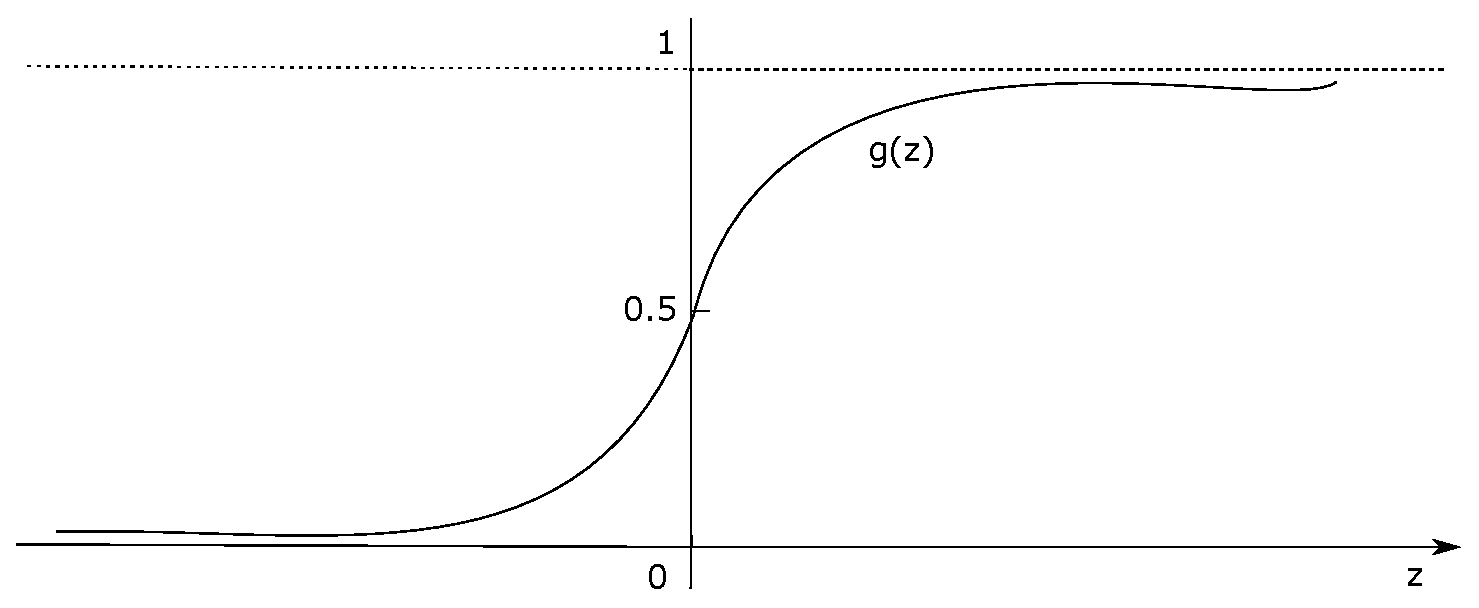
\includegraphics[height = 1.5in]{Images/sigmoid}
\end{center}

As we see on the plot, the sigmoid function maps any real number to the $(0, 1)$ interval, making it useful for transforming an arbitrary-valued function into a function better suited for classification.

\subsection*{Decision boundaries}

The equation \eqref{eq:log-reg-hyp} gives $h_\theta(x)$ as the estimated probability that $y=1$ given the input $x$ and the parameters $\theta$, so to get our binary classification, we can translate the output of the hypothesis function as follows:

\begin{align*}
  h_\theta(x) \geq 0.5 & \longrightarrow y =1 \\
  h_\theta(x) < 0.5 & \longrightarrow y = 0
\end{align*}

Since $h_\theta(x) = g(\theta^Tx)$, and looking on $g$ behaves on positive/negative numbers, we observe that $$h_\theta(x) = g(\theta^T x) \geq 0.5  \text{, if } \theta^T x \geq 0$$ and $$h_\theta(x) = g(\theta^T x) < 0.5  \text{, if } \theta^T x < 0.$$

Therefore:

\begin{align*}
  \theta^Tx \geq 0 & \longrightarrow y =1 \\
  \theta^Tx < 0 & \longrightarrow y = 0
\end{align*}

The line defined by $\theta^Tx = 0$ is called "decision boundary" and separates the area where $y = 0$ and where $y = 1$. Note that it depends only on the hypothesis function.

In general, we can consider more complex decision boundaries (polynomial, etc.) depending on the initial hypothesis we plug into the sigmoid function. For example, if we take $z = \theta_0 + \theta_1x_1^2 +\theta_2x_2^2$, then the decision boundary $\theta_0 + \theta_1x_1^2 +\theta_2x_2^2 = 0$ is a circle.

\subsection*{Cost function}

 We cannot use the same cost function that we use for linear regression because the logistic function will cause the output to have many local optima (in other words, it will not be a convex function).

Instead, we define the cost function for logistic regression as:

\begin{equation}\label{eq:log-reg-cost}
J(\theta) = \dfrac{1}{m} \sum_{i=1}^{m}{\cost(h_\theta(x^i), y^i)},
\end{equation}
where the cost of a single training example is given by:

$$\cost(h_\theta(x), y) = \left\{\begin{matrix}
                                    -\log(h_\theta(x)) & \text{, if } y = 1 \\
                                    -\log(1 - h_\theta(x)) & \text{, if } y = 0
                                  \end{matrix}\right.$$

This new cost function, defined by equation \eqref{eq:log-reg-cost}, is convex so we can apply gradient descent to find the optimal $\theta$.

\hspace{1.0in}

\begin{center}
\begin{minipage}{0.48\textwidth}
 \centering
 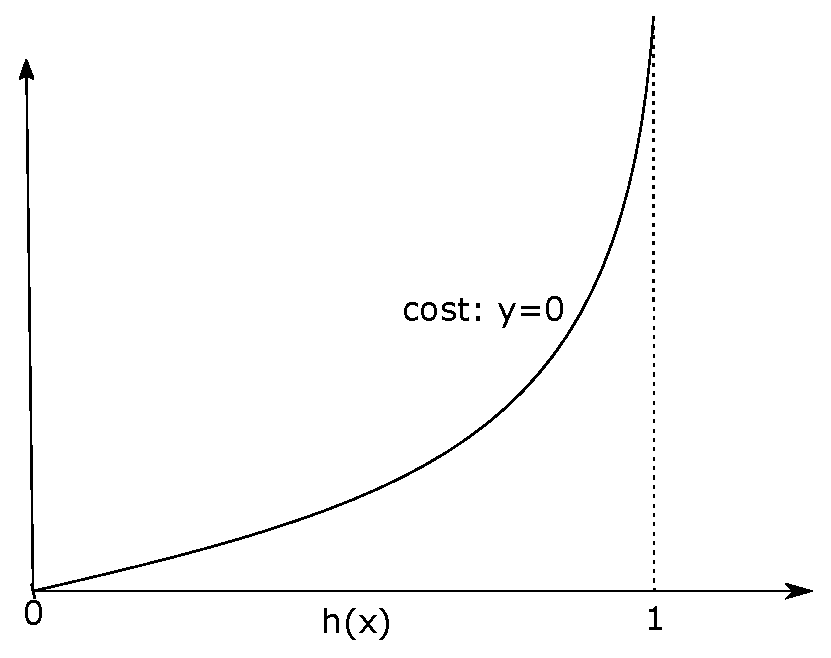
\includegraphics[width=.8\linewidth]{Images/cost_0}
 %\captionof*{figure}{Cost when y = 0}
\end{minipage}\hfill
\begin{minipage}{0.48\textwidth}
 \centering
 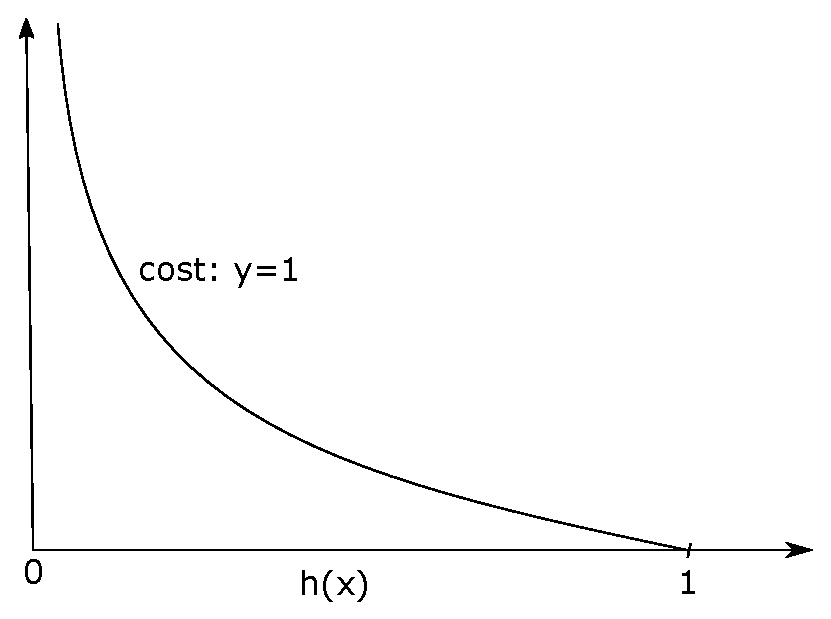
\includegraphics[width=.8\linewidth]{Images/cost_1}
 %\captionof*{figure}{Cost when y = 1}
\end{minipage}
\end{center}

Note that if $y = 1$ and $h_\theta(x) = 1$, then the $\cost$ will be $0$. If $y = 1$ and $h_\theta(x) \longrightarrow 0$ , then $\cost\longrightarrow \infty$, so wrong predictions are penalized by a very large cost (see figures).

\subsection*{Gradient descent}

 We can compress the cost function's two conditional cases into one case: $$\cost(h_\theta(x),y) = - y \; \log(h_\theta(x)) - (1 - y) \log(1 - h_\theta(x))$$

Notice that when $y$ is equal to $1$, then the second term $(1-y)\log(1-h_\theta(x))$ will be zero and will not affect the result. If $y$ is equal to $0$, then the first term $-y \log(h_\theta(x))$ will be zero and will not affect the result.

We can fully write out our entire cost function as follows:
\begin{equation}\label{eq:log-reg-cost2}
J(\theta) = - \frac{1}{m} \displaystyle \sum_{i=1}^m [y^{(i)}\log (h_\theta (x^{i})) + (1 - y^{i})\log (1 - h_\theta(x^{i}))],
\end{equation}
or vectorized as:
\begin{equation}\label{eq:log-reg-cost-vec}
J(\theta)  = \frac{1}{m} \cdot \left(-y^{T}\log(h)-(1-y)^{T}\log(1-h)\right),
\end{equation}
where $h = g(X\theta)$.

Remember the general form of gradient descent, as in \eqref{eq:lin-reg-gd}: $$\theta_j := \theta_j - \alpha \dfrac{\partial}{\partial \theta_j}J(\theta).$$

Computing the partial derivative for the cost function \eqref{eq:log-reg-cost2}, it turns out that the gradient decent equations for logistic regression look exactly the same as for linear regression:
$$\theta_j := \theta_j - \frac{\alpha}{m} \sum_{i=1}^m (h_\theta(x^{i}) - y^{i}) x_j^{i}.$$

A vectorized implementation of the gradient descent is given by: $$\theta := \theta - \frac{\alpha}{m} X^{T} (g(X \theta ) - {y}).$$

\subsection*{Multiclass classification: one-vs-all}

Assume that we have more than two classes in our classification problem, i.e. instead of having $y = \{0,1\}$, we have $y = \{0,1, \ldots, k\}$, with $k \geq 3$.
In this case, we divide our problem into $k+1$ binary classification problems; in each one, we predict the probability that $y$ is a member of one of our classes.

We have $k+1$ hypotheses $h_\theta^{(0)}, h_\theta^{(1)}, \ldots, h_\theta^{(k)}$, defined as:
\begin{align*}
h_\theta^{(0)}(x) &= P(y = 0 | x ; \theta), \\
h_\theta^{(1)}(x) &= P(y = 1 | x ; \theta), \\
\vdots &\\
h_\theta^{(k)}(x) &= P(y = n | x ; \theta), \\
\end{align*}
and we make the final prediction by taking:

$$h_\theta(x) := \max_{i\leq k} h_\theta ^{(i)}(x). \\$$

We are basically choosing one class and then lumping all the others into a single second class. We do this repeatedly, applying binary logistic regression to each case, and then use the hypothesis that returned the highest value as our prediction.


\section{Regularization}

\subsubsection*{Overfitting/underfitting}

High bias or underfitting is when the form of our hypothesis function $h$ maps poorly to the trend of the data. It is usually caused by a function that is too simple or uses too few features, e.g. if we take $h_\theta(x) = \theta_0 + \theta_1x_1 + \theta_2x_2$ then we are making an initial assumption that a linear model will fit the training data well and will be able to generalize but that may not be the case.

At the other extreme, overfitting or high variance is caused by a hypothesis function that fits the available data but does not generalize well to predict new data. It is usually caused by a complicated function that creates a lot of unnecessary curves and angles unrelated to the data.

This terminology is applied to both linear and logistic regression. There are two main options to address the issue of overfitting:

\begin{itemize}
\item Reduce the number of features:
    \begin{itemize}
      \item manually select which features to keep,
      \item use a model selection algorithm.
    \end{itemize}

\item Regularization: keep all the features, but reduce the parameters $\theta_j$.
\end{itemize}

Regularization is designed to address the problem of overfitting and works well when we have a lot of slightly useful features.

If our hypothesis function overfits the data, we can reduce the weight that some of the terms in our function carry by increasing their cost. Assume we have the following hypothesis:
$\theta_0 + \theta_1x + \theta_2x^2 + \theta_3x^3 + \theta_4x^4$ and we want to make more quadratic, i.e. we want to eliminate the influence of $\theta_3x^3$ and $\theta_4x^4$.

Instead of getting rid of these features or changing the form of the hypothesis, we can modify the cost function as such:

$$J(\theta) = \ds \dfrac{1}{2m}\sum_{i=1}^m (h_\theta(x^i) - y^{i})^2 + 1000\cdot\theta_3^2 + 1000\cdot\theta_4^2.$$

We add two extra terms at the end to inflate the cost of $\theta_3$ and $\theta_4$. Now, in order for the cost function to get close to zero, we have to reduce the values of $\theta_3$ and $\theta_4$ to near zero. This will in turn greatly reduce the values of $\theta_3x^3$ and $\theta_4x^4$ in our hypothesis function.

We can regularize all parameters at once and define a new cost function as:

\begin{equation}\label{eq:reg-cost}
J(\theta) = \ds \dfrac{1}{2m} \left[ \sum_{i=1}^m (h_\theta(x^{i}) - y^{i})^2 + \lambda \sum_{j=1}^n \theta_j^2 \right],
\end{equation}
where $\lambda > 0$ is the regularization parameter. By convention, the parameter $\theta_0$ is not regularized.

In fact $\lambda$ represents a trade-off between a good fit of the data and smaller parameters (a simpler hypothesis). If $\lambda$ is chosen to be too large, it may simplify the hypothesis too much and cause underfitting. Observe that the regularization term is actually equal to $\lambda \norm{\theta}_2^2$, where $\theta^T = [\theta_1, \ldots, \theta_n]$. One can also regularize by the term $\lambda \norm{\theta}_1^2$, and even by a combination of them: $\lambda_1 \norm{\theta}_1^2 + \lambda_2 \norm{\theta}_2^2$.

\subsection*{Regularized linear regression}

Assume that we regularize the cost function for linear regression as in \eqref{eq:reg-cost}. Then the gradient descent equations become:

\begin{equation}\label{eq:mul-reg-gdreg}
\begin{split}
\theta_0 := & \; \theta_0 - \alpha \dfrac{1}{m} \sum_{i=1}^m (h_\theta(x^{i}) - y^{i})x_0^{i}, \\
\theta_j := & \; \theta_j - \alpha \left[ \left( \dfrac{1}{m}\sum_{i=1}^m (h_\theta(x^{i}) - y^{i})x_j^{i} \right) + \frac{\lambda}{m}\theta_j \right], \; j\geq 2. \\
\end{split}
\end{equation}

Recall that $\theta$ can be also obtained as a solution of the normal equation \eqref{eq:mul-reg-neq}: $$\theta = (X^TX)^{-1}X^Ty.$$

One can prove that the regularized normal equation becomes: $$\theta = (X^TX +\lambda \cdot I)^{-1}X^Ty,$$
where $I$ is a $(n+1)\times (n+1)$ diagonal matrix with entries $(0,1,1,\ldots, 1)$. Actually, $I$ is very similar to the identity matrix $I_{n+1}$ except for the $(1,1)$ entry which is 0 in our case, since $\theta_0$ is not regularized.

We mentioned before that $X^TX$ may not be invertible if $m \leq n$. However, by adding the regularization term $\lambda\cdot I$, the matrix $X^TX +\lambda\cdot I$ becomes invertible.

\subsection*{Regularized logistic regression}

We can regularize logistic regression in a similar way as linear regression. Let's start with the regularized cost function:

\begin{equation}\label{eq:log-reg-costreg}
J(\theta) = - \dfrac{1}{m} \sum_{i=1}^m [ y^{i}\log (h_\theta (x^{i})) + (1 - y^{i}) \log (1 - h_\theta(x^{i}))\large] + \frac{\lambda}{2m}\sum_{j=1}^n \theta_j^2
\end{equation}
​	
The gradient descent equations are identical to \eqref{eq:mul-reg-gdreg}:

\begin{equation*}
\begin{split}
\theta_0 := & \; \theta_0 - \alpha \dfrac{1}{m} \sum_{i=1}^m (h_\theta(x^{i}) - y^{i})x_0^{i}, \\
\theta_j := & \; \theta_j - \alpha \left[ \left( \dfrac{1}{m}\sum_{i=1}^m (h_\theta(x^{i}) - y^{i})x_j^{i} \right) + \frac{\lambda}{m}\theta_j \right], \; j\geq 2. \\
\end{split}
\end{equation*}


\chapter{Neural Networks}

\section{Neural networks representation}

\subsection*{Non-linear hypotheses}

Performing linear regression with a complex set of data and many features is very unwieldy. Assume that we have 3 features and want to define a hypothesis that includes all the quadratic terms:
$$g(\theta_0 + \theta_1x_1^2 + \theta_2x_1x_2 + \theta_3x_1x_3 + \theta_4x_2^2 + \theta_5x_2x_3 + \theta_6x_3^2).$$

That gives us 6 features. If we start with 100 features and want to include all the quadratic terms, we get $5050$ resulting features.

One can approximate the growth of the number of new features we get with all quadratic terms with $\mathcal{O}(\dfrac{n^2}{2})$. If we want to include all cubic terms in our hypothesis, the number of features grows asymptotically at $\mathcal{O}(n^3)$. These are very steep growths, so as the number of our features increase, the number of quadratic or cubic features increase very rapidly and becomes quickly impractical.

For example, assume that the training set is a collection of $50 \times 50$ pixel B\&W photographs, and our goal will be to classify which ones are photos of cars. Our feature set size is then $n = 2500$ if we compare every pair of pixels. Now let's say we consider a quadratic hypothesis function. In this case, the total number of features will be about $2500^2 / 2 = 3125000$, which is very impractical.

Neural networks offers an alternate way to perform machine learning when we have complex hypotheses with many features.

\subsection*{Model representation}

At a very simple level, brain neurons are computational units that take input (dendrites) as electrical input which is channeled to outputs (axons).

We start from logistic regression and build an abstract representation of a neuron (also called logistic unit in this context). The inputs (dendrites) are the features $x_1, \ldots, x_n$, and the output (axon) is the result of the hypothesis function $h_\theta(x) = g(\theta^Tx)$. The components of a layer are called nodes or units.

\begin{center}
\begin{neuralnetwork}[height=4]
    \newcommand{\x}[2]{$x_#2$}
    \newcommand{\h}[2]{$h_\theta$}
    \newcommand{\ab}[2]{$z$}
    \newcommand{\linktheta}[4]{$\theta_#2$}
    \newcommand{\linkg}[4]{$g$}
    \inputlayer[count=2, bias=true, title=Input layer, text=\x]
    \outputlayer[count=1, text=\ab]
    \setdefaultlinklabel{\linktheta}
    \linklayers
    \outputlayer[count=1, title=Output, text=\h]
    \setdefaultlinklabel{\linkg}
    \linklayers
\end{neuralnetwork}
\captionof*{figure}{Neuron model (logistic unit)}
\end{center}

As before, we add an extra input node $x_0 = 1$, which is called "bias unit". The parameters $\theta_0, \theta_1, \ldots, \theta_n$ are now called "weights". We compute the output of the node $z$ by taking the weighted sum of the inputs, i.e. $z = \theta^Tx = \theta_0x_0 + \theta_1x_1 + \ldots + \theta_nx_n$.

To get the actual output $h_\theta(x)$ we apply the logistic (or sigmoid) function $g(z) = \dfrac{1}{1+\mathrm{e}^{-z}}$ to the node $z$ ($g$ is called the "activation function" of the node $z$), hence:
$$ h_\theta(x) = g(\theta^Tx) = \dfrac{1}{1 + \mathrm{e}^{-\theta^Tx}}.$$

The first layer is called the "input layer" and the final layer the "output layer," which gives the final value computed by the hypothesis. We can have intermediate layers of nodes between input and output, called "hidden layers." The nodes of a hidden layer are also called "activation units".

\begin{center}
\begin{neuralnetwork}[height=4]
    \newcommand{\x}[2]{$x_#2$}
    \newcommand{\au}[2]{$a^{#1}_#2$}
    \newcommand{\weights}[4]{$\theta^#3_{#4#2}$}
    % from layer=#1, from node=#2 to layer=#3, to node=#4
    \setdefaultlinklabel{\weights}
    \inputlayer[count=3, bias=true, title=Input, text=\x]
    \hiddenlayer[count=3, bias=true, title=Hidden, text=\au]
    \linklayers[title=$\Theta^1$]
    \outputlayer[count=1, title=Output, text=\au]
    \linklayers[title=$\Theta^2$]
\end{neuralnetwork}
\captionof*{figure}{Network with one hidden layer}
\end{center}

This figure describes a simple neural network with one hidden layer. The input layer has three units $x_1, x_2, x_3$, plus the bias unit $x_0=1$. The hidden layer has three nodes $a^1_1, a^1_2, a^1_3$, and as before we add a bias node $a^1_0=1$. Finally, we have one output node $a^2_1 = h_\Theta(x)$.

To map the input layer to the hidden layer we use a matrix of weights $\Theta^1 = \{\theta^1_{ik}\}\in\mathbb{R}^{3\times 4}$, where $k$ represents the starting node and $i$ represents the target node. Similarly, to map the hidden layer to the output layer we use a matrix of weights $\Theta^2 = \{\theta^2_{ik}\}\in\mathbb{R}^{1\times 4}$.

The values of the activation units $a^j_i$ are computed as follows:

\begin{equation}\label{eq:nn-act-nod}
\begin{split}
a_1^{1} = & g(\Theta_{10}^{1}x_0 + \Theta_{11}^{1}x_1 + \Theta_{12}^{1}x_2 + \Theta_{13}^{1}x_3), \\
a_2^{1} = & g(\Theta_{20}^{1}x_0 + \Theta_{21}^{1}x_1 + \Theta_{22}^{1}x_2 + \Theta_{23}^{1}x_3), \\
a_3^{1} = & g(\Theta_{30}^{1}x_0 + \Theta_{31}^{1}x_1 + \Theta_{32}^{1}x_2 + \Theta_{33}^{1}x_3), \\
& \\
h_\Theta(x) =  a_1^{2} = & g(\Theta_{10}^{2}a_0^{1} + \Theta_{11}^{2}a_1^{1} + \Theta_{12}^{2}a_2^{1} + \Theta_{13}^{2}a_3^{1}). \\
\end{split}
\end{equation}

The process of computing the values of all nodes starting from the input units is called "forward propagation".

Let's fix some notations we are going to use from now on:
\begin{align*}
x_i = & \text{ the input units, including the bias unit }, \\
s_j = & \text{ the number of units in layer $j$}, \\
a_i^j = & \text{ activation of unit $i$ in layer $j$}, \\
\Theta^j = & \text{ matrix of weights mapping layer $j-1$ to layer $j$}.
\end{align*}

Since we have $s_{j-1}$ units in layer $j-1$ and $s_{j}$ units in layer $j$, then the dimension of the matrix $\Theta^j$  is $s_{j}\times (s_{j-1}+1)$. The $+1$ comes from the addition of the bias nodes in the input.

\subsection*{Vectorized representation}

In this section we describe a vectorized implementation of the forward propagations equations.

We denote by $z^j_i$ the inputs of function $g$ in equations \eqref{eq:nn-act-nod}. More precisely:

\begin{equation}\label{eq:nn-def-z's}
\begin{split}
z_i^{1} = & \; \Theta_{i0}^{j}x_0 + \Theta_{i1}^{1}x_1 + \cdots + \Theta_{in}^{1}x_n,\; i=1,2,3, \\
z_1^{2} = & \; \Theta_{10}^{2}a_0^{1} + \Theta_{11}^{2}a_1^{1} + \Theta_{12}^{2}a_2^{1} + \Theta_{13}^{2}a_3^{1}. \\
\end{split}
\end{equation}

Considering vectors $x = [x_0, x_1, \ldots, x_n]^T$ and $z^j = [z^j_1, z^j_2, \ldots, z^j_n]^T$  and $x = a^0$, we can write: $$z^{j} = \Theta^{j} \cdot a^{j-1}, \; \text{ for each layer } j.$$

Recall that the matrix $\Theta^j$ has dimension $s_{j}\times (s_{j-1}+1)$, where $s_j$ is the number of activation nodes in layer $j$. The vector $a^{j-1}$ has $s_{j-1}+1$ elements, so the resulting vector $z^{j}$ has $s_j$ elements.

Having this in hand, we can write the activation nodes for layer $j$ as follows: $$a^{j} = g(z^{j}),$$ where $g$ is applied element-wise to the vector $z^{j}$. After computing $a^{j}$, we then add a bias unit $a_0^{j} = 1$ to layer $j$.

If $j+1$ is the output layer, to compute our hypothesis, we first have: $$z^{j+1}=\Theta^{j+1}\cdot a^j.$$
Since $\Theta^{j+1}$ has dimension $s_{j+1}\times (s_{j}+1)$, $a^j$ has $s_j + 1$ elements and $s_{j+1} = 1$, we get that $z^{j+1}$ is just a real number.
Finally: $$h_\Theta(x) = a^{j+1} = g(z^{j+1}).$$


\subsubsection*{Example 1}

A simple example of applying neural networks is by predicting the output of a logical operator \verb"AND" which returns \verb"TRUE" if and only if both arguments are \verb"TRUE".

We use simple network with no hidden layers:

\begin{center}
\begin{neuralnetwork}[height=4]
    \newcommand{\x}[2]{$x_#2$}
    \newcommand{\h}[2]{$h_\Theta(x)$}
    \inputlayer[count=2, bias=true, text=\x]
    \outputlayer[count=1, text=\h]
    \linklayers[title=$\Theta^1$]
\end{neuralnetwork}
\end{center}

Remember that $x_0$ is the bias input and is always equal to 1. Setting $$\Theta^1 := [−30, 20, 20],$$ we have: $$h_\Theta(x) = g(-30 + 20x_1 + 20x_2).$$

More explicitly, we get the following cases:
\begin{align*}
x_1 = 0 \text{ and } x_2 = 0  \longrightarrow h_\Theta(x) = &\; g(-30) \sim 0 \\
x_1 = 0 \text{ and } x_2 = 1  \longrightarrow h_\Theta(x) = &\; g(-10) \sim 0 \\
x_1 = 1 \text{ and } x_2 = 0  \longrightarrow h_\Theta(x) = &\; g(-10) \sim 0 \\
x_1 = 1 \text{ and } x_2 = 1  \longrightarrow h_\Theta(x) = &\;\;\;\; g(10)  \sim 1 \\
\end{align*}
So we have built one of the fundamental operations in computers by using a small neural network rather than using an actual \verb"AND" gate.

\subsubsection*{Example 2}

Neural networks can also be used to simulate all the other logical gates. The weights matrix for \verb"OR"  is $[-10, 20, 20]$ and for \verb"NOR" is $[10, -20, -20]$.
We can combine these to get the \verb"XNOR" logical operator, which returns 1 if $x_1$ and $x_2$ are both 0 or both 1.

\begin{center}
\begin{neuralnetwork}[height=4]
    \newcommand{\x}[2]{$x_#2$}
    \newcommand{\au}[2]{$a^{#1}_#2$}
    \newcommand{\h}[2]{$h_\Theta(x)$}
    \inputlayer[count=2, bias=true,text=\x]
    \hiddenlayer[count=2, bias=false, text=\au]
    \linklayers[title=$\Theta^1$]
    \outputlayer[count=1, text=\h]
    \linklayers[title=$\Theta^2$]
\end{neuralnetwork}
\end{center}

To map the input layer to the hidden layer, we use a $\Theta^1$ matrix that combines the values for \verb"AND" and \verb"NOR":
$$\Theta^{(1)} =\begin{bmatrix}-30 & 20 & 20 \\ 10 & -20 & -20\end{bmatrix}.$$

To map the hidden layer to the output layer, we use the $\Theta^2$ matrix of \verb"OR": $$\Theta^{(2)} =\begin{bmatrix}-10 & 20 & 20\end{bmatrix}.$$

One can easily check that this simple network with one hidden layer indeed implements the operator \verb"XNOR".

\subsection*{Multiclass Classification}

To classify a set of data into multiple classes, we allow our hypothesis function to return a vector of values. Assume that we want to classify our data into one of the four resulting classes:

\begin{center}
\begin{neuralnetwork}[height=5.5]
    \newcommand{\x}[2]{$x_#2$}
    \newcommand{\au}[2]{$a^{#1}_#2$}
    \newcommand{\h}[2]{${h_\theta}_#2$}
    %\newcommand{\weights}[4]{$\theta^#3_{#4#2}$}
    % from layer=#1, from node=#2 to layer=#3, to node=#4
    %\setdefaultlinklabel{\weights}
    \inputlayer[count=5, bias=true, title=Input, text=\x]
    \hiddenlayer[count=4, bias=true, title=Hidden, text=\au] \linklayers
    \hiddenlayer[count=4, bias=true, title=Hidden, text=\au] \linklayers
    \outputlayer[count=4, title=Output, text=\h] \linklayers
\end{neuralnetwork}
\captionof*{figure}{Network with many hidden layer}
\end{center}

The final hidden layer, when multiplied by its $\Theta$ matrix, will map to a vector on which we apply the sigmoid function $g$ to get the final vector of hypothesis values.


\section{Neural networks learning}

\subsection*{Cost function}

Remember from the previous section that, for a neural network, we denote by $L$ total number of layers in the network, by $s_j$ the number of units (not counting the bias unit) in layer $j$ and by $K \geq 1$ the number of output units/classes. We denote by $h\Theta(x)_k$ the hypothesis that results in the $k$-th output.

We have seen in the previous section that a neural network looks locally like a logistic regression. The cost function we use for training neural networks is going to be a generalization of the cost function for logistic regression. Recall from \eqref{eq:log-reg-costreg} the cost function for regularized logistic regression:
$$ J(\theta) = - \dfrac{1}{m} \sum_{i=1}^m \large[ y^{i}\ \log (h_\theta (x^{i})) + (1 - y^{i})\ \log (1 - h_\theta(x^{i}))\large] + \frac{\lambda}{2m}\sum_{j=1}^n \theta_j^2.$$

For neural networks, the cost function is going to be slightly complicated:

\begin{equation}\label{eq:nn-cost}
\begin{split}
J(\Theta) = & - \dfrac{1}{m} \sum_{i=1}^m \sum_{k=1}^K \left[y^{i}_k \log ((h_\Theta (x^{i}))_k) + (1 - y^{i}_k)\log (1 - (h_\Theta(x^{i}))_k)\right] + \\
            & + \dfrac{\lambda}{2m}\sum_{l=1}^{L-1} \sum_{i=1}^{s_{l-1}} \sum_{j=1}^{s_{l}} \left( \Theta_{ji}^{l}\right)^2
\end{split}
\end{equation}

The first part of the equation \eqref{eq:nn-cost} looks similar to \eqref{eq:log-reg-costreg}, and additionally  we sum up over $K$, the number of the output nodes.

The regularization term includes all the weights that appear along the network. Recall that the dimension of $\Theta^l$ is $s_l \times (s_{l-1}+1)$, but since we do not regularize the bias weights, we actually have that $\Theta^l$ is $s_l \times (s_{l-1})$ dimensional.


\subsection*{The backpropagation algorithm}

The backpropagation algorithm is a method of computing the partial derivatives of the cost function of a neural network, to use further in gradient descent. Our goal is to find an optimal set of weights $\Theta$ that minimize the cost function $J$ from \eqref{eq:nn-cost}.

Recall that for gradient descent we have to compute the partial derivatives $\dfrac{\partial}{\partial\Theta^l_{ji}}J(\Theta)$ and update the parameters accordingly at each iteration.

In the case of backpropagation, we compute the "error" $\delta_j^{l}$ of every node $j$ from layer $l$, starting with the last layer. Recall that $a_j^l$ denotes the activation of unit $j$ in layer $l$.

For the output layer, we have that: $$\delta^{L} = a^{L} - y,$$
where $L$ is the number of layers and $a^{L}$ is the vector of outputs of the activation units of the last layer. So the "error" values for the output layer are simply the differences of the nodes in the output layer and the correct values in $y$.

To get the errors of the layers before the output layer, we use an equation that steps us back from right to left: $$\delta^{l} = (\Theta^{l})^T \delta^{l+1}\ .*\ g^\prime(z^{l}),$$
where $z^l$ is defined by \eqref{eq:nn-def-z's} and $g^\prime$ is the derivative of $g$.
The errors of layer $l$ are calculated by multiplying the errors in the next layer with the matrix of weights of layer $l$. We then multiply this element-wise ($.*$) with the derivative of the activation function $g$ evaluated in $z^l$.

One can prove that the derivative of $g$ can be written as $g^\prime(u) = g(u)\ .*\ (1 - g(u))$. Then the backpropagation equation for nodes in layer $l$ becomes:

\begin{equation}\label{eq:nn-bkprp-eq}
\delta^{l} = (\Theta^{l})^T \delta^{l+1}\ .*\ a^{l}\ .*\ (1 - a^{l}).
\end{equation}

Ignoring regularization, one can prove that the partial derivatives of the cost function $J$ are given by:
\begin{equation}\label{eq:nn-cost-deriv}
\dfrac{\partial J(\Theta)}{\partial \Theta_{ij}^{l}} = \dfrac{1}{m}\sum_{t=1}^m a_j^{t,l} {\delta}_i^{t,l+1}.
\end{equation}

Notice that $\delta^{l+1}$  and $a^{l+1}$ are vectors with $s_{l+1}$ elements. Similarly, $a^{l}$ is a vector with $s_l$ elements. Multiplying them produces a matrix that is $s_{l+1}$ by $s_l$ which is the same dimension as $\Theta^l$. That is, the process produces a gradient term for every element in $\Theta^l$.

TODO: check correct dimensions!

We can now take all these equations and put them together into an algorithm.

\subsubsection*{The backpropagation algorithm}

Assume we have a training set ${(x^1,y^1), \ldots, (x^m,y^m)}$, with $m$ observations.
\begin{description}
\item[Step 1]{Set $\Delta^{l}_{ij}:= 0$, for all indices $l, i, j$.}

\item[Step 2] {For each training example $t$:

\begin{itemize}
\item set $a^{1} := x^{t}$,
\item do forward propagation to compute $a^{l}$, for $l=2,3,\ldots,L$,
\item using $y^{t}$, compute $\delta^{L} = a^{L} - y^{t}$,
\item compute $\delta^{L-1}, \delta^{L-2},\ldots, \delta^{2}$, using the backpropagation equation \eqref{eq:nn-bkprp-eq},
\item update $\Delta^{l}_{ij} := \Delta^{l}_{ij} + a_j^{l} \delta_i^{l+1}$.
\end{itemize}
}
\item[Step 3]{Compute $D^l_{ij} := \dfrac{1}{m}\left(\Delta^l_{ij} + \lambda\Theta^l_{ij} \right)$, if $j\neq 0$, and $D^{l}_{ij} := \dfrac{1}{m}\Delta^{l}_{ij}$, if $j = 0$.}

\item[Step 4]{Compute $\dfrac{\partial}{\partial\Theta^l_{ji}}J(\Theta) = D^l_{ij}$, for all indices $l, i, j$.}
\end{description}

Now we have all necessary ingredients to train a neural network.

\subsection*{Training a neural network}

\begin{enumerate}
  \item Choose a network architecture (layers, outputs, units, etc.):
    \begin{itemize}
      \item number of input units = number of features,
      \item number of output units = number of classes,
      \item take one hidden layer as default, or many hidden layers with the same number of units.
    \end{itemize}

  \item Randomly initialize the weights set $\Theta$ (with small values near 0).

  \item Implement forward propagation to compute the output of the hypothesis $h_\Theta$ for all inputs.

  \item Implement the cost function $J(\Theta)$ and implement backpropagation to compute its partial derivatives with respect to all weights $\Theta^l_{ij}$:

    For each training example $(x, y)$:
    \begin{itemize}
      \item do forward propagation to compute the activations $a^l$, for all layers $l$,
      \item do backpropagation to compute the errors $\delta^l$,
      \item update $\Delta^l := \Delta^l + \delta^{l+1}(a^l)^T$ and compute the partial derivatives of $J(\Theta)$.
    \end{itemize}

  \item Use an optimization algorithm (e.g. gradient descent) to find parameters $\Theta$ which minimize the cost function $J(\Theta)$.
\end{enumerate}


\chapter{Model Evaluation}

\section{Evaluating a hypothesis}

A hypothesis may have low error on the training examples, but large error when we try to predict on new examples (because of overfitting). With a given dataset of training examples, we can split up the data into two parts: a training set and a test set, and use them both in the learning process:
\begin{itemize}
\item learn $\theta$ by minimizing $J(\theta)$ on the training set,
\item compute the $J_{\mathrm{test}}(\theta)$ on the test set and compare.
\end{itemize}

For linear regression, the test set error is defined by: $$J_{\mathrm{test}}(\theta) = \dfrac{1}{2m_{\mathrm{test}}}\sum_{i=1}^{m_{\mathrm{test}}}{(h_\theta(x^i_{\mathrm{test}})−y^i_{\mathrm{test}})^2}.$$
For classification problems, we can use the misclassification error:
$$\mathrm{error}(h_\Theta(x),y) =
\left\{\begin{matrix}
1, & \text{ if }  h_\Theta(x) \geq 0.5 \text{ and } y = 0 \text { or } h_\Theta(x) < 0.5  \text{ and } y = 1, \\
0, & \text{ otherwise,}\\
\end{matrix}\right.$$
and then average over the test set:
$$ \text{test error} = \dfrac{1}{m_{\mathrm{test}}} \sum^{m_{\mathrm{test}}}_{i=1} \mathrm{error}(h_\Theta(x^{i}_{\mathrm{test}}), y^{i}_{\mathrm{test}}).$$
This formula gives us the proportion of the test data that was misclassified.

\section{Model selection}

Just because a learning algorithm fits a training set well, that does not mean it is a good hypothesis. The error of a hypothesis as measured on the dataset used to learn the parameters will be lower than on any other dataset.

For example, assume that we have a hypothesis $h_\theta(x)$ which is a polynomial of degree $d$. We can split the initial dataset into training/testing sets and do the following:
\begin{itemize}
  \item optimize $\theta$ on the training set, for each value of $d$,
  \item find the degree $d$ giving the lowest error on the test set,
  \item estimate the generalization error of $h_{\theta, d}$ on the test set.
\end{itemize}
This is a bad method because we learn $d$, the degree of the polynomial hypothesis, using the test set and this will cause our error to be greater for any other set of new data.

To solve this issue, we use an intermediate set to learn $d$, called "cross-validation" set. Typically, we split the initial training set into three parts:
\begin{enumerate}
  \item Training set: $\sim 60\%$ of the data, used to learn several hypotheses $h_\theta(x)$,
  \item Cross-validation set: $\sim 20\%$ of the data, used to test all hypothesis learned and choose the best one,
  \item Testing set: $\sim 20\%$ of the data, used to estimate the generalization error.
\end{enumerate}

\subsection*{Bias vs. Variance}

Most of the time, our models will suffer of one of the following problems:
\begin{description}
  \item[High bias/Underfitting:] the model/hypothesis is too simple to fit the data, and both training and cross-validation error are high
  \item[High variance/Overfitting:] the model/hypothesis is too complex, the training error is small and the cross-validation error is large.
\end{description}

\begin{center}
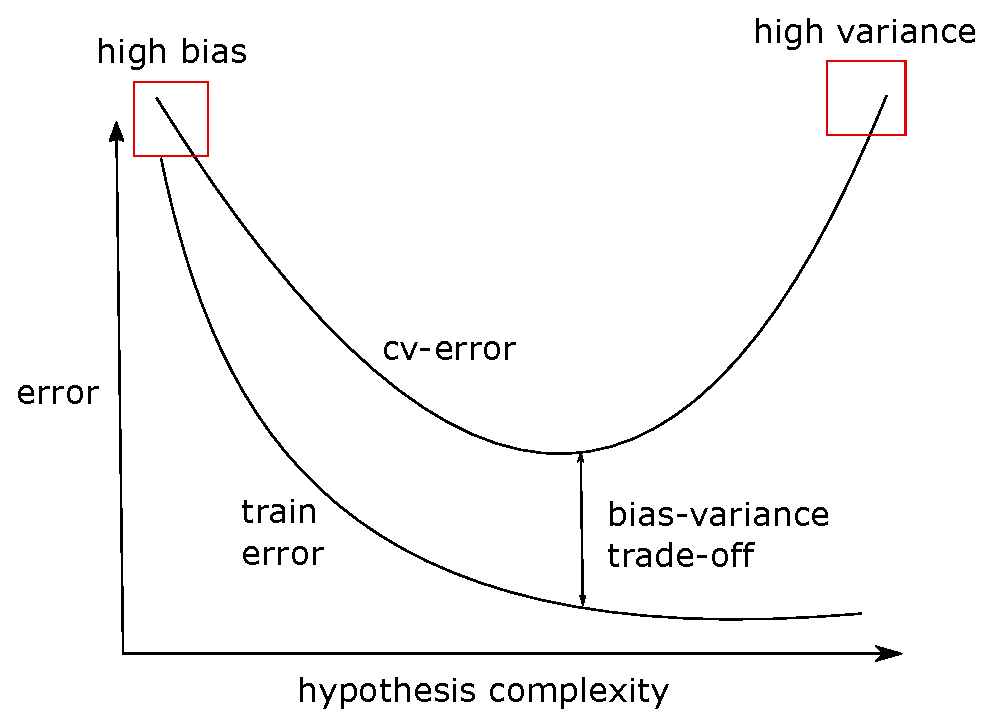
\includegraphics[height = 2in]{Images/bias_variance}
\end{center}

If we use a regularized cost function, then choosing a very large parameter $\lambda$ may cause high bias and choosing a very small $\lambda$ may cause high variance. To find the optimal $\lambda$ we use the cross-validation set.

\begin{center}
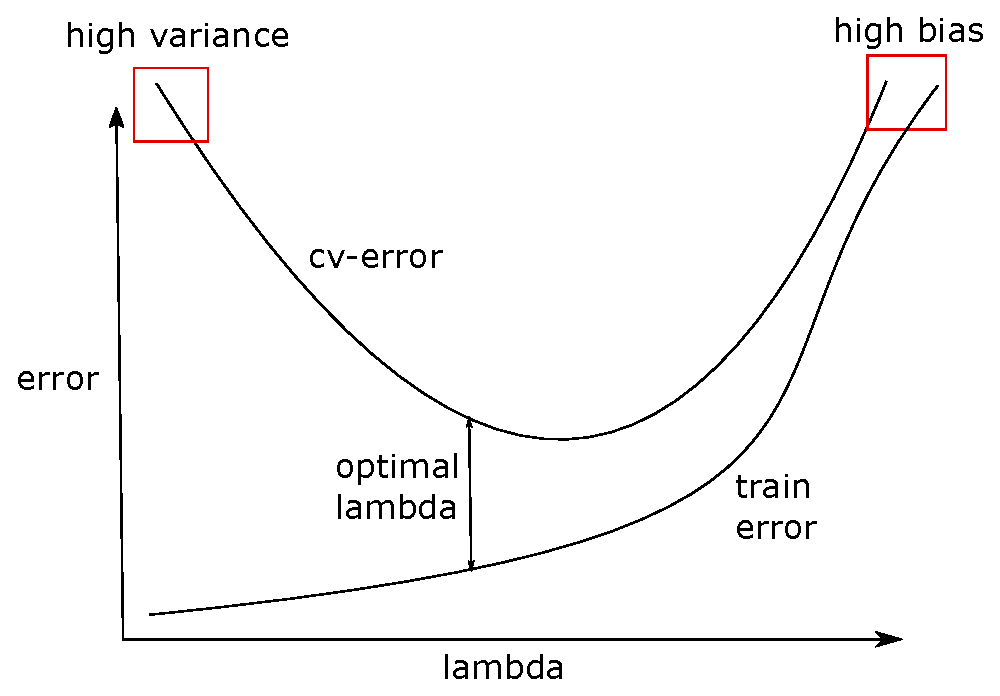
\includegraphics[height = 2in]{Images/bias_variance_lambda}
\end{center}

\subsection*{Learning curves}




















\begin{center}
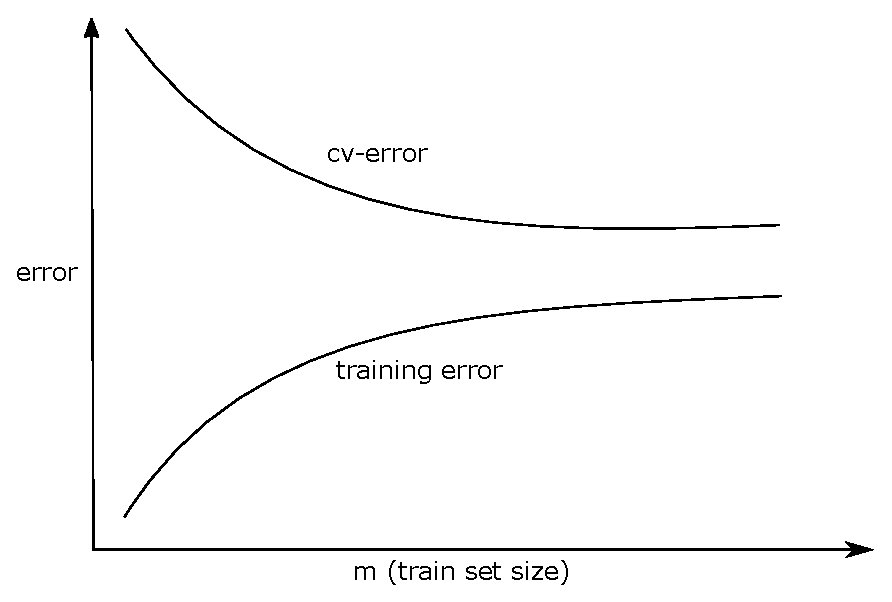
\includegraphics[height = 2in]{Images/learn_curve}
\end{center}
































































\end{document}
